%%%%%%%%%%%%%%%%%%%%%%%%%%%%%%%%%%%%%%%%%%%%%%%%%%%%%%%%%%%%%%%%%%%%%%%%%%%%%%
% EXAME DE QUALIFICAÇÃO
% ALUNO: 
% ORIENTADOR: 
%%%%%%%%%%%%%%%%%%%%%%%%%%%%%%%%%%%%%%%%%%%%%%%%%%%%%%%%%%%%%%%%%%%%%%%%%%%%%%

\documentclass[12pt]{article}

\usepackage[english]{babel}
\usepackage[utf8]{inputenc}
\usepackage{ae,url,enumerate}
\usepackage{indentfirst}
\usepackage[numbers,sort]{natbib}
\usepackage{graphicx,epsfig}
\usepackage{epstopdf}
\usepackage{longtable}
\usepackage[table]{xcolor}
\usepackage{setspace,fancybox}
\usepackage[paperwidth=210mm,paperheight=297mm,margin=20mm]{geometry}
\usepackage{textgreek}
\usepackage{amssymb,amsmath}
\usepackage{easyReview}

\setreviewson


% definindo alguns comandos de uso frequente (test git)
\newcommand\hi{\hspace*{\parindent}}
\newcommand\vi{\vspace{\baselineskip}}
\newcommand{\up}[1]{\raisebox{1.5ex}[0pt]{#1}}
\newcommand{\changed}[1]{{\color{red}#1}} % na versão final, basta alterar a cor para "black"


% Erros de separacao silabica
\hyphenation{ResUnet-a}


\setlength {\marginparwidth }{2cm}
\begin{document}



	\thispagestyle{empty}
	\singlespacing

    \indent
	\ovalbox{
		\begin{minipage}{0.8\linewidth}
			{\Large\bf Federal University of São Carlos}\\
			{\sc Graduate Program in Computer Science}\\
			{\sc School of Management \& Technology}
		\end{minipage} \hfill 
		
		\begin{minipage}{0.12\linewidth}
				\epsfxsize=2.5cm
				\centerline{\epsffile{ufscar_logo.eps}}
		\end{minipage}
	}

	\vfill
	\vi
	\vi
	\vi

	\begin{center}
		\Large Master's Project

		\Large Graduate Program in Computer Science

		\vfill

		\Large Qualification Exam\\

	\end{center}

	\vi

	\begin{center}
	    \LARGE\bf Crop field detection using graph-based image segmentation and contrastive learning
	    %\LARGE\bf Crop field detection using graph-based image segmentation with contrastive learning
		%\LARGE\bf Combining graph-based image segmentation with contrastive learning for automatic crop field detection
	\end{center}

	\vfill

	\begin{center}
		{\bf Candidate:}~Eduardo Garcia do Nascimento\footnote{E-mail: \texttt{egnascimento@gmail.com} | Lattes: \url{http://lattes.cnpq.br/1693471368947954}}

		{\bf Advisor:}~Prof. Dr. Tiago A. Almeida\footnote{E-mail:
		\texttt{talmeida@ufscar.br} | Lattes: \url{http://lattes.cnpq.br/5368680512020633}}
	\end{center}

	\vfill
	\vfill

	\begin{center}
		February 2022 to January 2024
	\end{center}

	\vfill

	\newpage
	\baselineskip=1.38\baselineskip
	\setcounter{page}{1}

\section*{Abstract}

As the world population grows, the motivation to ensure enough food for everyone has brought a diversity of technologies from other industries to agriculture. The main challenge is producing more food with fewer resources using a collection of techniques known as precision agriculture. In precision agriculture, drawing crop field boundaries is an essential practice, and it allows the farmer to evaluate operating performance separately and compare different seed varieties, pesticides, and fertilizers. However, manually drawing field boundaries is often a deep time-consuming task. In this context, we propose a method to detect crop fields automatically and infer their boundaries by applying graph-based image segmentation combined with contrastive learning, an approach that achieves comparable performance to supervised deep learning methods but without requiring a massive amount of labeled samples.

\section{Introduction}\label{section:introduction}

% Session 1: Introduce the meaning of precision agriculture
Food production needs to grow by 70\% to meet the food demands of the expected world population by 2050~\cite{nelson2010}. Motivated by this challenge, agriculture has adopted technologies primarily developed for other areas to improve and optimize returns on inputs while preserving natural resources. Integrating these technologies promotes a farming management concept known as \textit{precision agriculture}~\cite{zhang2002}. The main goal of precision agriculture is to provide tools to allow the farmer to observe, measure, and respond to field variability in crops facilitating faster and better decisions. In addition, this collection of techniques is generic enough to be applied to a diversity of crops, including but not limited to corn, soy, coffee, sugarcane, beans, and even pastures~\cite{mulla2013,bhakta2019}.

% Session 2: Talk about the crop fields and their main purpose
In order to efficiently organize and manage large crops, farmers leverage remote sensing to divide their land into smaller observation units that this work will refer to as \textit{agricultural} or \textit{crop fields}. A field shape is designed based on topography and mechanization planning. For example, fields are built around contour farming and the ideal length to fill the wagon capacity in a sugarcane crop. In Brazilian South and Southeast, the same logic is followed for grains. Nonetheless, the most important variable is the harvester capacity in the Midwest, where the topography is often plain~\cite{spekken2015,griffel2019,bolfe2020}.

% Session 3: Talk about the challenge
% Session 3.1: Challenge of doing stuff manually
Usually, farmers rely on experts to build the field boundaries in a dedicated Geographic Information Systems (GIS) software (e.g., QGIS\footnote{QGIS -- a free and open source geographic information system. Available at: \url{https://qgis.org/en/site/}. Access on July 10, 2022.}). Despite the expert's ability and knowledge, drawing the boundaries of agricultural plots has been a major, error-prone, and time-consuming challenge~\cite{wagner2020}. The larger the customer's land is, the more significant the number of fields to be created. According to the marketing department at John Deere\footnote{We have obtained this information directly from the John Deere employees in June 2022}, there are farms in Brazil with more than eighteen thousand fields that require regular updates to reflect their accurate states. 

In Figure~\ref{figure:fieldanalyzer}, a field analyzer software demonstrates the variability inside a crop field. The areas of the field are colored with gradients from green to red, proportional to the productivity. For example, areas in red had the lowest productivity, while areas in green had the highest. This information helps farmers understand how to improve their operations by comparing this data with seed varieties, fertilizers, and machine operations. These are some of the motivations behind the delineation of field boundaries: define the area for evaluating supplies, machines, and techniques to improve crop productivity.

\begin{figure}[ht]
\centering
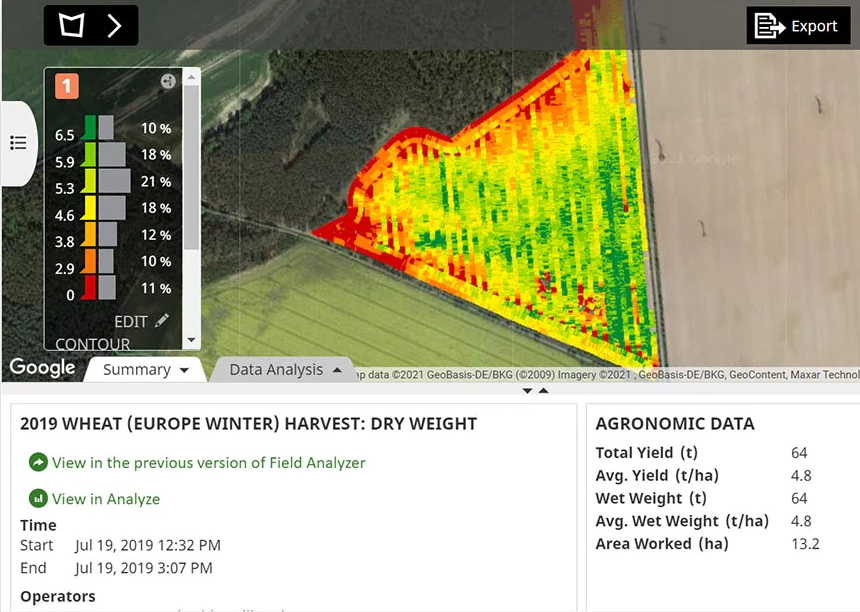
\includegraphics[height=8cm]{Projeto de Qualificação - Eduardo/res/field-analyzer.png}
\caption{\label{figure:fieldanalyzer}Agriculture field analyzer\protect\footnotemark}
\end{figure}
\footnotetext{Field analyzer. Available at: \url{http://salesmanual.deere.com/sales/salesmanual/en_NA/ams/2017/feature/wdt_field_analyzer.html}. Access on July 10, 2022.}

% Session 3.2: Suggest doing it automatically and talk about the challenges
Given a map provided by remote sensing techniques, a method to automatically detect crop fields represents a significant improvement in the agriculture management sector~\citep{garcia2017,garcia2018,garcia2019}. However, seasonal changes and the crop type add some challenges to detecting these fields from remote sensing, even to the naked eye, due to variations reflected in the images over the year~\citep{north2019}. Moreover, the different sizes and shapes can create additional difficulties demanding various scenarios to consider. For example, Ukrainian fields are often much more large than South African ones. North American sugarcane fields also have much more regular shapes than equivalent fields in Brazil~\cite{waldner2020}. Furthermore, when creating a robust automatic detection method, it is also important to give attention to clouds and other noises inherent to the extraction methods ~\citep{graesser2017,north2019}. Additionally, the within-field variance can be greater than the between-field variance in remote sensing~\cite{evans2002}.

Fortunately, some automatic and semi-automatic methods have been proposed to outline the boundaries of agricultural fields. Edge-based approaches detect boundaries with reasonably good accuracy however fail when forming closed polygons~\cite{taravat2021,waldner2021}. Region-based methods are more successful when producing closed polygons, but often do not place boundaries at the visible edges~\cite{taravat2021}. There is a significant increase in efficiency in hybrid methods where both edge and region approaches are combined~\cite{garcia2017}. However, both methods and combinations have not been successful in images with high within-field variance~\cite{mueller2004,zhang2021}.

Deep learning-based approaches are the current state-of-the-art when dealing with these challenges~\citep{waldner2021,zhang2021}. However, they require massive sets of labeled samples often unavailable in real-case scenarios~\cite{kokkinos2016, ma2019,kamilaris2018}. 
% Briefly explain the proposal
To overcome this limitation, we propose applying contrastive learning to detect the similarity of connected pixels to delineate crop fields using the well-known graph-based image segmentation, i.e., components of an image are connected by an edge whose weight is proportional to the similarity between them~\citep{felzenszwalb2004}. Contrastive learning is a method capable of achieving deep learning equivalent results requiring a limited amount of labeled data. Although it has been successfully applied to agricultural images~\cite{guldenring2021,jansel2021}, this work proposes, in an unprecedented way, leveraging similar approaches for the automatic detection of agricultural fields. We hypothesize that using a self-supervised or semi-supervised method should overcome the limitations of obtaining sufficient training data~\citep{yang2020}. Additionally, requiring a smaller amount of labeled samples gives us better control over its quality.

The remainder of this project is organized as follows. In Section~\ref{section:bibliografia}, we present the main related work. The hypothesis and main objectives are described in Section~\ref{section:objetivos}. Section~\ref{section:constrastive-learning} describes the proposed approach. In Section~\ref{section:materiais}, we detail the materials and methods required for the whole development of this project. Finally, the work plan is presented in Section~\ref{section:planotrabalho}.

\section{Bibliographical context}\label{section:bibliografia}

% Reminder of the challenge and its importance before start talking about the previous related work
Automatic detection of crop fields is a challenge that intersects multiple areas, and its solution could fill important gaps in agriculture management and environment control~\citep{bolfe2020}. In this context,~\citet{crommelinck2019} has worked on boundary detection of agricultural fields to provide automated recording of land rights, a slightly different purpose despite sharing common problems. However, despite the proven benefits of fully automated boundary detection and the research already accomplished, it is still considered an open problem with significant innovation opportunities, especially when sufficient training data is not available~\citep{waldner2021,yang2020}.

% Start describing the evolution and previous work
\citet{north2019} used classic computer vision to detect the boundaries of farm fields in New Zealand. However, their technique resulted in only 59\% accuracy, which is insufficient for most applications. Moreover, their strategy is highly impacted by variations caused by the season the images were extracted.


% Deep learning work from the Polytechnic University, Spain
Since computer vision alone is often not enough to achieve good results, further research evaluated machine learning to detect crop boundaries. For instance, \citet{garcia2017} achieved an accuracy of 92\% using an ensemble algorithm called RUSBoost~\citep{seiffert2010} to merge superpixels and group blocks of the image part of the same field. This study demonstrated how machine learning is a promising alternative and a precursor to further development using deep learning~\citep{garcia2017}. Two years later, \citet{garcia2019} proposed the U-Net, a convolutional neural network for semantic image segmentation, to perform the same task with improved performance~\cite{garcia2017,garcia2018,garcia2019}.

% Deep learning work from the University of Twente, Netherlands
Concurrently, \citet{persello2019} designed a deep learning approach using SegNet, a convolutional network architecture commonly used for semantic segmentation in Very High Resolution (VHR) images. In SegNet, only the pooling indices are transferred to the expansion path from the compression path using less memory. In contrast, in UNet, entire feature maps are transferred from compression path to expansion path, demanding much more memory. Both techniques attained remarkable performance. However, some significant mistakes were generally associated with poor-quality training data~\citep{persello2019}. As deep learning requires a tremendous amount of training data, it is difficult to assure its quality. The authors extend their work on medium-resolution images from Sentinel-2, using two different deep learning architectures, SRC-Net and MD-FCN. Again, they observed a severe limitation during training since these methods comprised many convolutional layers resulting in a time-consuming task~\cite{persello2019,masoud2020}.

% Edge-based that was later improved with deep learning from Kiel University, Germany
\citet{wagner2020} designed a modified version of the growing snakes active contour model based on graph theory concepts~\cite{wagner2020}. This technique, referred to as graph-based growing contour, can extract complex networks of boundaries in agricultural landscapes requiring little supervision. Evaluated on rural area maps, it detected 99\% of total acreage, but it achieved a poor performance close to urban areas. In sequence, \citet{wagner2020.2} integrated a deep learning technique into their already proven graph-based model. For this, a fully connected MLP-NN was used to make a pixel-wise prediction of whether it was a boundary. The method achieved excellent results in rural areas but required further investigation of the missed boundaries, especially in areas closer to the cities~\cite{wagner2020.2,wagner2020}.

%Another graph-based approach was presented by~\citet{alshehhi2017}. It applies graph-based segmentation focused in roads detection, however, agricultural fields can be implied depending on the scenario. There is limited diversity of road patterns which is one of the reasons why this work falls short on addressing the challenge of field detection. It is also suggested in this paper the need of a more efficient algorithm because the combination of sequential merging and splitting methods and Dijkstra require additional computations depending on the image~\citep{alshehhi2017}.

% Deep learning work from the European Commission Join Research Center
\citet{waldner2020} compared deep learning methods starting with ResUnet-a and followed by an improvement named Fractal-ResUNet, a network designed for the task of semantic segmentation of agricultural images. It employs hierarchical watershed segmentation, a technique that relies on graph theory, suggesting this as a successful approach to address the image segmentation challenge of crop fields. The experiments presented the best accuracies with Sentinel-2 images, and it is considered the state-of-the-art in boundary detection of agricultural fields. However, it strongly depends on a large amount of training data with high-quality labeling to achieve consistent results~\cite{waldner2020,waldner2021}.

% In the last paragraph I emphasize 2 important things:
% 1. Graph-theory for segmentation is a trend in the latest successful research, including the state-of-the-art. 
% 2. The challenge of working with limited samples still remains unsolved.
% With these two important points, I finish the bibliographic review with what could represent a meaningful contribution and it is also what this work suggests.

% Start reviewing contrastive learning to be more specific on the method
It has been continuously observed that, in deep learning methods, data availability is usually a limitation. This challenge motivates a different approach with less dependency on large amounts of data. Latest advances in the area suggest self-supervised and semi-supervised methods, more precisely, using contrastive learning as a promising alternative~\cite{guldenring2021}. %In that sense, this work proposes the evaluation, in an unprecedented way, of contrastive learning for detecting crop fields in scenarios with scarce labeled data.
In the next section, we briefly explain how contrastive learning works.

\section{Constrastive learning}\label{section:constrastive-learning}

Contrastive learning allows a model learning to maximize the agreement between two differently augmented images. Samples are compared and pushed towards each other if they belong to the same distribution. On the other hand, they are pulled against each other if belonging to different distributions~\cite{chen2020}.

This method does not depend on high-quality labeled data, whose acquisition is costly in many scenarios. Moreover, even with softened requirements, the results achieved by self-supervised and semi-supervised contrastive learning may be equivalent to supervised methods~\citep{chen2020}.

The learning pipeline is usually built with three main steps: data augmentation, encoding, and similarity measurement~\citep{ashish2020}. Figure~\ref{figure:contrastive_learning} shows these three steps and the attraction and repelling process at the end.

\begin{figure}[ht]
\centering
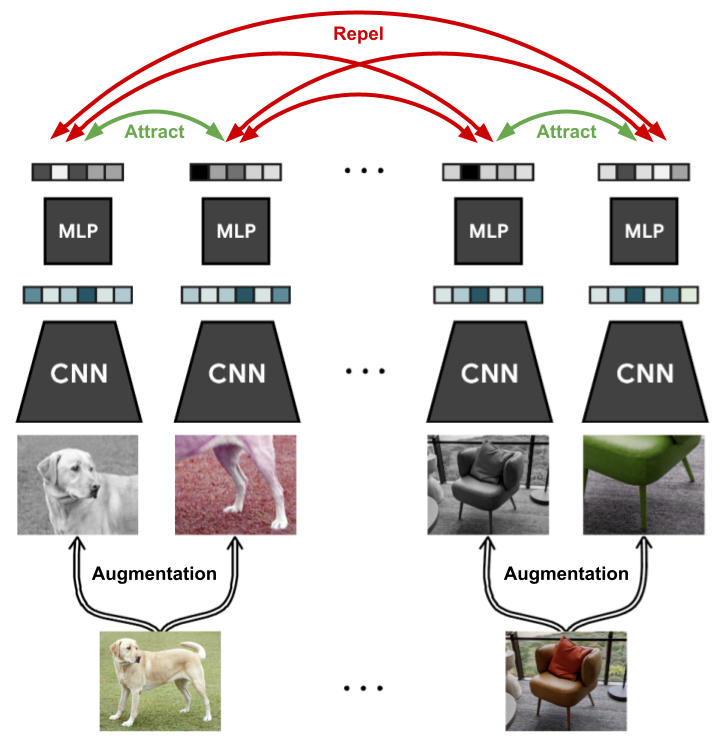
\includegraphics[height=7cm]{res/contrastive_learning}
\caption{\label{figure:contrastive_learning}Contrastive learning architecture~\citep{ashish2020}}
\end{figure}

% Step 1: Data Augmentation
A stochastic data augmentation module randomly creates two correlated views of the same sample. These views are the positive pairs denoted ${\tilde{\boldsymbol{x}_i}}$ and $\tilde{\boldsymbol{x}_j}$. Three augmentations are applied in the following sequence: random cropping, random color distortions, and random Gaussian blur. This process extends the number of positive samples and figures the most crucial hyper-parameter in contrastive learning~\citep{chen2020}.

% Step 2: Encoding
The second step is encoding. This module is a neural network-based encoder $f(\cdot)$ that extracts the vector representations from all the augmented images. There is no restriction on the choice of the encoder's architecture. However, due to its simplicity, a ResNet-50~\citep{zhang2016} model is generally preferred for various implementations, including SimCLR~\citep{chen2020}. Other implementations use a few layers of convolutional neural networks instead to benefit speed, such as NNCLR~\citep{dwibedi2021}. ResNet, in this case, is used to obtain $ \boldsymbol{h}_i=f(\tilde{\boldsymbol{x}_i})=ResNet(\tilde{\boldsymbol{x}_i})$, where $\boldsymbol{h}_i$ is the output after the average pooling layer.

% Step
%Finally, in the third and last step, the vector representations are passed to a projection head for the last stage of processing. In this particular case, it is an MLP (Multi Layer Perceptron) with only one hidden layer. This MLP is only used during training and refining of the input images. Once it is completed, the result is processed by a loss function that attracts similar samples while repealing those that are not part of the same cluster. By applying the contrastive loss and clustering the samples, it is achieved the classification that has been compared to supervised methods in terms of accuracy but with much lower requirements during the data preparation phase. 
Finally, the vector representations are processed by a projection head $g(\cdot)$ , represented by a Multi-Layer Perceptron (MLP) with one hidden layer. This module is used to compute $\boldsymbol{z}_i = g(\boldsymbol{h}_i) = \boldsymbol{W}^{(2)}\sigma(\boldsymbol{W}^{(1)}\boldsymbol{h}_i)$, where $\sigma$ is a ReLU nonlinearity. This is employed for training and refining the input images. Once completed, the loss function is used to attract similar samples while repealing those not part of the same cluster. By applying the contrastive loss and clustering the samples, the classification performance has been compared to supervised methods in terms of accuracy, even requiring a much lower amount of labeled data~\citep{chen2020}.

% The contrastive loss, which aims to pull close representations and push away different representations, is given by Equation~\ref{eqn:contrastive_learning}. In the case of SimCLR, a contrastive loss called NT-Xent Loss (Normalised temperature scaled cross entropy) is used, however, other loss functions can be used depending on the implementation. 
% Firstly, the augmented pairs are taken one by one. A similarity function gets the probability of these two images to be part of the same cluster. This comparison is represented in the numerator of the Equation~\ref{eqn:contrastive_learning}. Secondly, in the denominator, there is the calculation of the similarity between the the samples and the negative pairs. The parameter \texttau~indicates the temperature or the strength of penalty applied during training. This value is empirically chosen and it has been seen, in previous works~\citep{chen2020,caron2020}, associated with values from 0.05 to 100. Finally, the loss is calculated with the negative of the log of the result of this division.
The contrastive loss is given by Equation~\ref{eqn:contrastive_learning}. It aims to pull close representations and push away different ones. In the case of SimCLR, a contrastive loss called NT-Xent Loss (Normalised temperature scaled cross entropy) is used. However, other loss functions can be used depending on the implementation. Firstly, the augmented pairs ($\tilde{\boldsymbol{x}}_i$ and $\tilde{\boldsymbol{x}}_j$) are taken one by one, and a similarity function computes the probability of these two images being part of the same cluster. This comparison is represented in the numerator of Equation~\ref{eqn:contrastive_learning}. Secondly, the denominator computes the similarity between the samples and the negative pairs. Finally, the parameter \texttau~indicates the temperature or the strength of penalty applied during training. Its value is empirically chosen, and previous studies have associated it with values from 0.05 to 100~\citep{chen2020,caron2020}. %Finally, the loss is calculated with the negative log of this division's result.

\begin{equation}
l_{(i,j)}=-\log{\frac{\exp{\left(\boldsymbol{z}_i\cdot\boldsymbol{z}_j/\tau\right)}}{\sum_{k=1}^{2N}\mathbf{1}_{i\neq k}\cdot\exp{\left(\boldsymbol{z}_i\cdot\boldsymbol{z}_k/\tau\right)}}}
\label{eqn:contrastive_learning}
\end{equation} 

\vspace{1.5em}

In terms of the history, \citet{chopra2005} introduced one of the first applications with  of contrastive learning using the loss calculation for face recognition. This study was later used as a base for the development of FaceNet~\citep{schroff2015}, a widely recognized approach to address this challenge. Other more generic implementations were further explored in the last few years, such as AMDIM~\citep{bachman2019}, MoCo~\citep{he2020}, and SimCLR~\citep{chen2020}.

% Talk about AMDIM
\citet{bachman2019} proposed a breakthrough implementation based on an idea five years before by~\citet{dosovitskiy2016}, where an original image was used to generate two others by applying data augmentation. This implementation, called AMDIM, designed a pipeline that was later used by two significant studies on the same area: MoCo~\citep{he2020} and SimCLR~\citep{chen2020}.

% Talk about Moco from Facebook
Later, Facebook proposed MoCo~\citep{he2020} using a similar strategy adopted by AMDIM but keeping the history of all batches to increase the number of negative samples.
% Talk about SimCLR
In turn, \citet{chen2020} developed the implementation considered the state-of-the-art in contrastive learning, called SimCLR. This study presented the best accuracies, equivalent to supervised methods when using the right number of parameters. The second version proposed by the authors presents essential improvements~\citep{chen2020.2}, including the memory mechanism initially proposed by MoCo~\citep{he2020}.

Based on the recent advances and successful implementations, \citet{saunshi2022} have introduced an inductive bias to contrastive learning models. Moreover, they have proved the existence of gaps in understanding how the algorithm works and the need to mathematically fill them in future research to accelerate progress in the area.

%Alternatively to contrastive learning, one-shot~\citep{fei2006} and few-shot~\citep{wang2020} learning-based approaches are also often mentioned as good candidates to overcome the lack of large volumes of high-quality labeled data to detect boundaries of crop fields automatically.

%Given the recent remarkable results presented by contrastive learning, with some of them compared to supervised methods, we expect that it will also perform satisfactorily when applied to detect crop fields with just a few labeled samples. This has the potential to overcome the well-known limitations of supervised deep learning-based approaches and, therefore, enable its application in real-world scenarios. To conclude, it is also important to highlight that, to the best of our knowledge, no similar studies investigate contrastive learning methods to detect crop fields in satellite images.

%\subsection{Graph-based image segmentation}\label{section:graph-segmentation}

% 

% HIPÓTESE E OBJETIVOS
\section{Hypothesis and objectives}\label{section:objetivos}

Given the recent remarkable results presented by contrastive learning, with some of them compared to supervised methods, we expect that it will also perform satisfactorily when applied with the established graph-based image segmentation approaches to detect crop fields with just a few labeled samples. This has the potential to overcome the well-known limitations of supervised deep learning-based methods and, therefore, enable its application in real-world scenarios. Moreover, to our knowledge, no similar studies combine contrastive learning with graph-based techniques to detect crop fields automatically.

We hypothesize that state-of-the-art methods with contrastive learning can be combined with graph-based segmentation to automatically detect crop fields requiring a reduced amount of high-quality labeled data, consequently allowing their application in real scenarios.

Therefore, the main objective of this project is to evaluate if contrastive learning combined with graph-based segmentation is a promising alternative to established deep learning models, able to detect crop fields automatically but requiring few labeled training samples. 

% PROPOSTA

\section{Proposal}\label{section:proposal}

This research project proposes an approach that automatically detects crop fields requiring just a few labeled samples. It can be divided into three main steps: data processing, training the contrastive learning model and graph-based image segmentation, as explained below.

\subsection{Data processing}\label{subsection:dataprocessing}

The first step is collecting the multi-temporal Sentinel-2 imagery and combine them with machine information. The machine information provides typical agricultural operations such as tillage, spraying and harvesting. Therefore, we can define crop field areas or positive samples from them, e.g., the brightest yellow part in Figure~\ref{figure:data_processing}. 

\begin{figure}[ht]
\centering
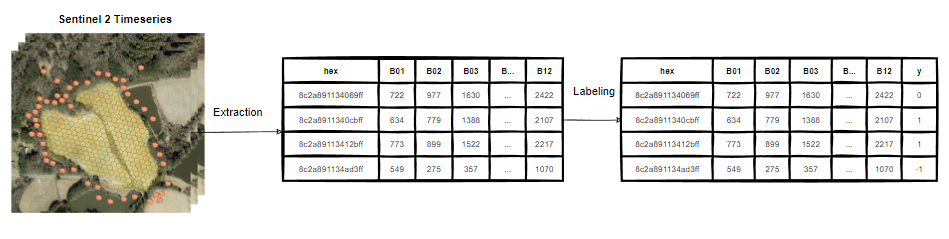
\includegraphics[width=17cm]{Projeto de Qualificação - Eduardo/res/dataprocessing.png}
\caption{\label{figure:data_processing}Data processing}
\end{figure}

The negative samples are defined by the areas where machines have not worked. Moreover, we propose to select some points near the inferred crop fields boundary for negative samples, e.g., the orange dots in Figure~\ref{figure:data_processing}. With this, we aim to maximize the dissimilarity with the positive samples, leading to algorithm efficiency improvements. Furthermore, we plan to group pixels as hexagons and seek regular grids with smooth gradients and equidistant neighbors. In addition, using hexagons rather than individual pixels may improve the speed during the next steps.

\subsection{Training the contrastive learning model}\label{subsection:cltraining}

% Describe how we plan the implementation
Once images and their respective labels are appropriately organized in the dataset, we plan to train the representation model using contrastive learning. Figure~\ref{figure:contrastive_training} illustrates its main steps.

\begin{figure}[ht]
\centering
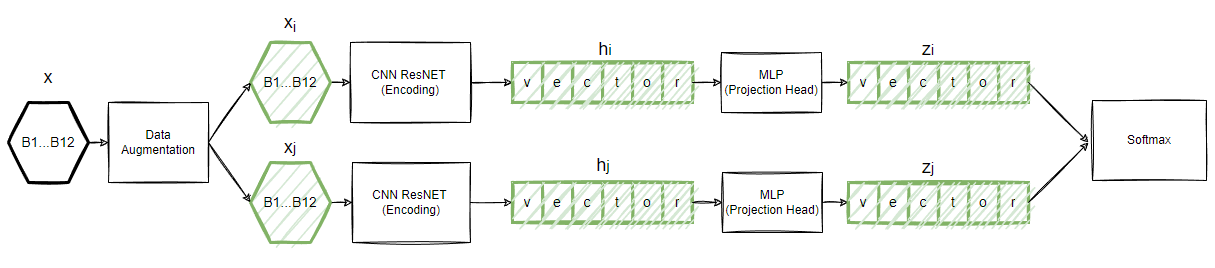
\includegraphics[width=17cm]{Projeto de Qualificação - Eduardo/res/clmodeltraining.png}
\caption{\label{figure:contrastive_training}Training the contrastive learning model}
\end{figure}

A slight perturbation will be applied to the original data to produce augmented data $\tilde{\boldsymbol{x}_i}$. The augmented pairs will be encoded to $\tilde{\boldsymbol{h}_i}$ by a convolutional neural network, and its output processed by a projection head to generate $\tilde{\boldsymbol{z}_i}$. The similarity of the output vectors $\tilde{\boldsymbol{z}_i}$ will be measured using cosine similarity, followed by calculating the probability of samples being part of the same class using softmax (Equation ~\ref{eqn:softmax}).

\begin{equation}
softmax=\frac{\exp{\left(sim(\boldsymbol{z}_i\cdot\boldsymbol{z}_j)/\tau\right)}}{\sum_{k=1}^{2N}\mathbf{1}_{i\neq k}\cdot\exp{\left(sim(\boldsymbol{z}_i\cdot\boldsymbol{z}_k)/\tau\right)}}
\label{eqn:softmax}
\end{equation}

We can interpret these probabilities as the likelihood of two neighboring samples being part of the same class. Therefore, as discussed in the next section, we can use them to create a graph to represent the image.

\subsection{Graph-based image segmentation}\label{subsection:graphbasedsegmentation}

We will create a graph where the nodes are the pixels of the image, and the edge weights are the likelihood of the two connected nodes being part of the same class, i.e., the probabilities computed by softmax. Therefore, we can employ established graph-based image segmentation techniques~\citep{felzenszwalb2004} to compute graph cuts~\citep{veksler2001} to distinguish field and non-field pixels in the map. The lowest probabilities identify the field boundary, i.e., the line that separates two different groups of classes, as highlighted in bold red in Figure~\ref{figure:hexgraph}.


\begin{figure}[ht]
\centering
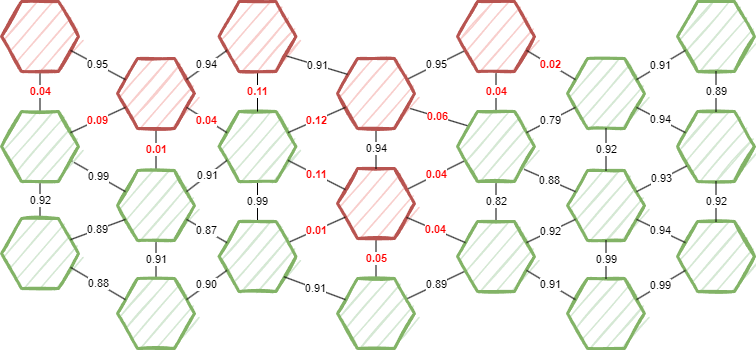
\includegraphics[width=11cm]{Projeto de Qualificação - Eduardo/res/hexgraph.png}
\caption{\label{figure:hexgraph}Graph-based image segmentation with similarity probabilities computed by softmax\protect}
\end{figure}

This technique can be applied to either group of hexes or pixels depending on the required precision and speed.


\section{Materials and methods}\label{section:materiais}

% Describe first remote sensing source
We will extract the remote sensing images from Sentinel-2 satellites to leverage its 10m precision and the variety of bands provided. Moreover, the multi-temporal acquisition should address possible noisy samples affected by the presence of clouds, for example. We also plan to use different layers to improve the model's performance since, with the right combination, we can identify the presence of water and other elements not belonging to the actual crop fields.

% Describe next how we are planning to get labels
We will collect a minimal amount of labeled data from a real database after data is appropriately anonymized. John Deere will provide this data in which the crop field boundaries are manually drawn by human specialists and may differ in quality. During the evaluation of the results, if we observe that poor quality label impacts the results, we can also estimate crop boundaries from machine operation data, assuming that these machines worked to the exact extents of the crop field.

We will implement the pixels clustering in hexagons with H3\footnote{H3 -- Hexagonal hierarchical geospatial indexing system. Available at: \url{https://h3geo.org/}. Access on September 24, 2022.} library support, a geospatial indexing system developed by Uber.


% Describe metrics
To validate the results, we plan to follow the metrics traditionally used by state-of-the-art supervised methods. They refer to field boundary detection, but there is an intimate connection with crop detection since we can easily infer its boundaries by finding a crop field. These metrics are often divided into thematic and geometric accuracies.

In thematic accuracies~\citep{lizarazo2014}, we have:
\begin{itemize}
    \item Pixel-based or Region-based accuracy: percentage of accurately classified pixels or agglomerated regions, depending on the used strategy;
    \item Overall, user's and producer's accuracy; and
    \item Matthew's correlation coefficient (MCC): an effective solution for imbalanced datasets.
\end{itemize}

In geometric accuracies~\citep{lizarazo2014}, we can use the following metrics:
\begin{itemize}
\item Boundary similarity: compares the boundary of the reference object with the classified one;
\[
S_{boundary}=\left({\frac{l_{intersection}}{pti}}\right)^k
\]
\item Location similarity: evaluates the similarity of the reference object with the classified one;
\[ 
S_{location}=1-\frac{d(C_{t_i};C_{E_j})}{D_{cac}}
\]
\item Over and under segmentation rates: how often multiple fields are detected where there is only one or a field is detected where there are two or more, respectively.
\end{itemize}

By evaluating the predicted results with these metrics, we will have enough data to compare them with well-established benchmarks and understand how this proposal performs compared to them.

\section{Work plan and timeline}\label{section:planotrabalho}

In the following, we present a list of activities executed and planned to complete this project and the execution timeline presented in Table~\ref{table:cronograma}.

\begin{enumerate}
	\item Credits required by PPGCC-So.

\begin{center}
	\begin{tabular}{|l|c|}
		\hline
		\textbf{Course} & \textbf{Grade} \\ \hline
		Aprendizado de Máquina & A \\ \hline
		Processamento de Imagens e Sensoriamento Remoto & A \\ \hline
		Teoria da Computação & A \\ \hline
		Robôs Móveis Autônomos & B \\ \hline
		Engenharia de Software & A \\ \hline
		Tópicos em Bancos de Dados & A \\ \hline
		Metodologia de Pesquisa Científica em Computação & A \\ \hline
	\end{tabular}
\end{center}	

	\item Bibliographical review;
	\item Data acquisition and processing: extraction of remote sensing images and manually drawn boundaries;
	\item Method implementation: implementing the state-of-the-art SimCLR and possibly other similar contrastive learning methods;
	\item Model training including required adaptations in the pipeline;
	\item Representing the images as graphs and evaluating graph-based image segmentation techniques to detect crop fields;
	\item Writing the dissertation and scientific research papers.

\begin{center}
    \begin{longtable}{|c|c|c|c|c|c|c|c|c|c|c|c|c|c|}
    \caption{Timeline with the executed activities (black), in development (dark grey) and planned (light grey).}\label{table:cronograma}\\   
    \hline
    & \multicolumn{4}{c|}{2022} & \multicolumn{4}{c|}{2023} \\
    \cline{2-10}
    \up{Activities} & 1\textordmasculine Trim. & 2\textordmasculine Trim. & 3\textordmasculine Trim. & 4\textordmasculine Trim. 
	& 1\textordmasculine Trim. & 2\textordmasculine Trim. & 3\textordmasculine Trim. & 4\textordmasculine Trim.\\
    \hline
    1&\cellcolor[gray]{.1}&&&&&&&\\
    \hline
    2&\cellcolor[gray]{.1}&\cellcolor[gray]{.4}&\cellcolor[gray]{.8}&\cellcolor[gray]{.8}&\cellcolor[gray]{.8}&\cellcolor[gray]{.8}&\cellcolor[gray]{.8}&\cellcolor[gray]{.8}\\
    \hline
    3&&\cellcolor[gray]{.4}&\cellcolor[gray]{.8}&\cellcolor[gray]{.8}&&&&\\
    \hline
    4&&\cellcolor[gray]{.4}&\cellcolor[gray]{.8}&\cellcolor[gray]{.8}&&&&\\ 
    \hline
    5&&&&\cellcolor[gray]{.8}&\cellcolor[gray]{.8}&\cellcolor[gray]{.8}&&\\   
    \hline
    6&&&&&\cellcolor[gray]{.8}&\cellcolor[gray]{.8}&\cellcolor[gray]{.8}&\\
    \hline
    7&&&&&&\cellcolor[gray]{.8}&\cellcolor[gray]{.8}&\cellcolor[gray]{.8}\\
    \hline
    \end{longtable}
\end{center}


\end{enumerate}


\bibliographystyle{natbib}
\bibliography{references.bib}


\end{document}